\chapter{Proton NMR}\label{ch:g12:proton-nmr}

In a hospital, a patient lies inside the ring of an MRI scanner, and an
image of the soft tissues of the body appears on the screen, built from
the answers of the hydrogen nuclei of its water and fats. In a chemistry
laboratory, a small glass tube holding a few milligrams of a compound is
lowered into the bore of a powerful magnet, and a spectrum appears built
the same way: a strong magnet, a radio signal, and hydrogen nuclei
answering it. In the chemist's spectrometer each hydrogen \omterm{def:g9:inside-the-atom:nucleus}{nucleus} answers
a little differently according to its neighbours, and the spectrum is a
map of the hydrogen \omterm{def:g7:atoms-and-molecules:atom}{atoms} of the \omterm{def:g7:atoms-and-molecules:molecule}{molecule}.

\begin{recall}
An \omterm{def:g11:infrared:spectrum}{infrared spectrum} shows which bonds a \omterm{def:g7:atoms-and-molecules:molecule}{molecule} contains
(\cref{ch:g11:infrared}). \omterm{def:g11:functional-groups:functional-group}{Functional groups}, families and \omterm{def:g11:organic-skeletons:isomer}{isomers}
(\cref{ch:g11:functional-groups}, \cref{ch:g11:organic-skeletons}).
\end{recall}

\begin{omfigure}
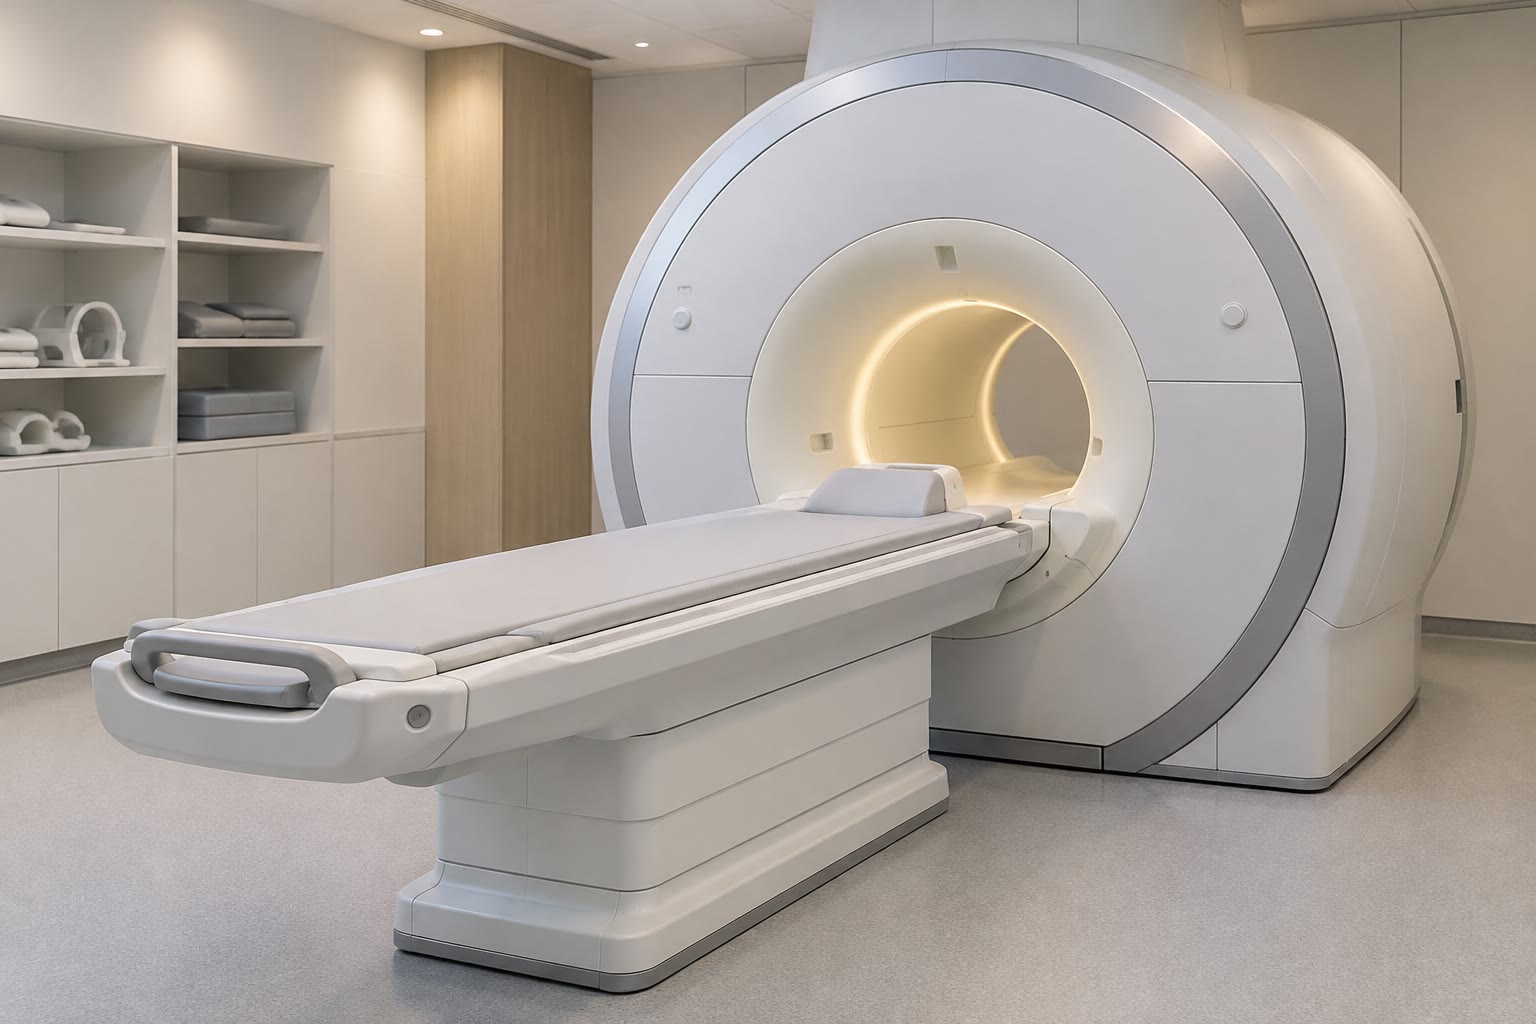
\includegraphics[width=0.48\linewidth]{images/book1/ai/g12-mri-room.jpg}

{\small An MRI scanner: the same physics as the chemist's NMR
spectrometer.}
\end{omfigure}

\section{Protons in a magnetic field}

The \omterm{def:g9:inside-the-atom:nucleus}{nucleus} of a hydrogen \omterm{def:g7:atoms-and-molecules:atom}{atom} is a single \omterm{def:g9:inside-the-atom:proton}{proton}. Placed in a strong
magnetic field, it absorbs radio waves of a precise frequency; how and
why belongs to physics, and is not needed here. What matters to the
chemist is that the \omterm{def:g9:inside-the-atom:nucleus}{electrons} around a \omterm{def:g9:inside-the-atom:proton}{proton} shield it slightly from the
field, and that this shielding depends on the \omterm{def:g7:atoms-and-molecules:atom}{atoms} nearby: a \omterm{def:g9:inside-the-atom:proton}{proton} next
to an electronegative oxygen \omterm{def:g7:atoms-and-molecules:atom}{atom}, which pulls \omterm{def:g9:inside-the-atom:nucleus}{electrons} away, absorbs at
a slightly different frequency from a \omterm{def:g9:inside-the-atom:proton}{proton} in a hydrocarbon chain. The
differences are tiny, a few millionths of the frequency, and are given
in parts per million.

\begin{omfigure}
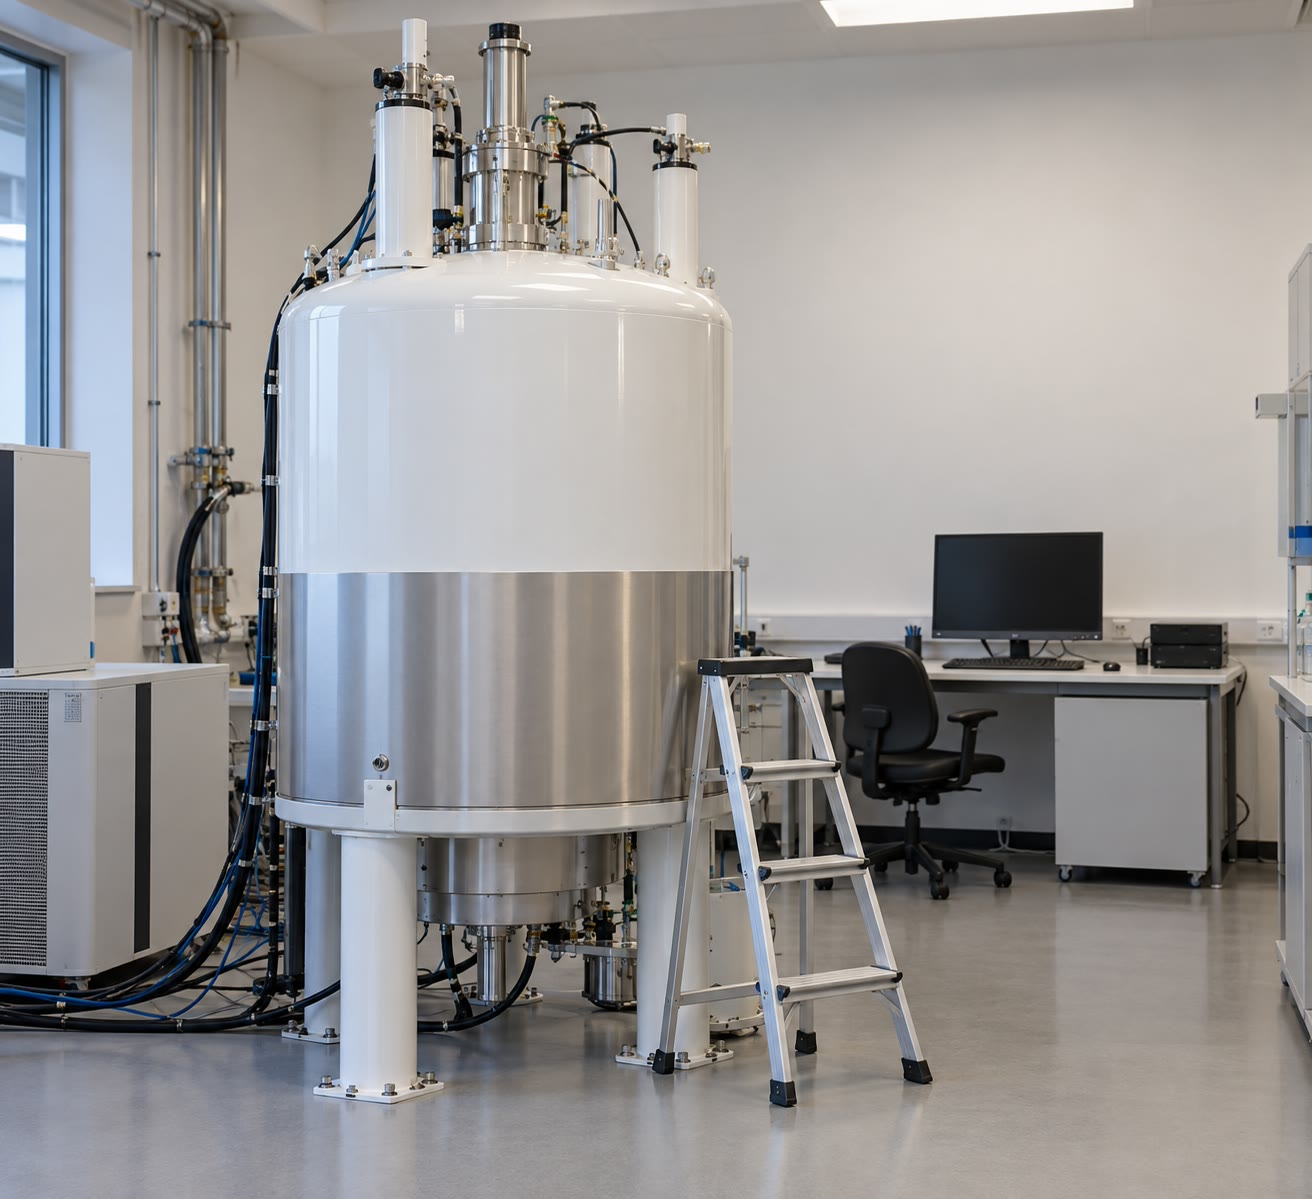
\includegraphics[width=0.42\linewidth]{images/book1/ai/g12-nmr-magnet.jpg}

{\small The magnet of an NMR spectrometer.}
\end{omfigure}

\begin{definition}[NMR spectrum, chemical shift]\label{def:g12:proton-nmr:spectrum}
A \omterm{def:g9:inside-the-atom:proton}{proton} \emph{NMR spectrum}\index{NMR spectrum} (nuclear magnetic
resonance) shows the signals absorbed by the hydrogen nuclei of a
compound. The position of a signal is its \emph{chemical
shift}\index{chemical shift} $\delta$, in parts per million (\si{ppm}),
measured from the signal of a reference compound, tetramethylsilane
\ce{Si(CH3)4} (TMS), set at $\delta = 0$. The $\delta$ axis is drawn
increasing from right to left.
\end{definition}

\begin{proposition}[The shift depends on the neighbours]\label{prop:g12:proton-nmr:shift}
% ledger: nmrr:CH3, nmrr:CH2, nmrr:allylic, nmrr:ketone, nmrr:halide, nmrr:alcohol, nmrr:vinylic, nmrr:aryl, nmrr:aldehyde, nmrr:acid
The \omterm{def:g12:proton-nmr:spectrum}{chemical shift} of a \omterm{def:g9:inside-the-atom:proton}{proton} depends on the \omterm{def:g7:atoms-and-molecules:atom}{atoms} close to it: the
nearer it is to an electronegative \omterm{def:g7:atoms-and-molecules:atom}{atom} or a \omterm{def:g10:lewis-and-shape:multiple-bond}{double bond}, the larger its
shift. Typical ranges, in \si{ppm}:
\begin{center}
\small
\begin{tabular}{ll@{\qquad}ll}
\hline
environment & $\delta$ & environment & $\delta$ \\
\hline
\ce{CH3} in a chain & 0.7--1.3 & \ce{H-C-O} (\omterm{def:g11:functional-groups:alcohol}{alcohol}, ether, \omterm{def:g11:functional-groups:carboxylic-acid}{ester}) & 3.3--4.5 \\
\ce{CH2} in a chain & 1.2--1.6 & \ce{H-C=C} & 4.5--6.5 \\
\ce{H-C-C=C} & 1.6--2.2 & H on a benzene ring & 6.5--8.0 \\
\ce{H-C-C=O} & 2.0--2.4 & \omterm{def:g11:functional-groups:carbonyl}{aldehyde} \ce{-CHO} & 9.7--10.0 \\
\ce{H-C-X} (\omterm{def:g10:electron-shells:family}{halogen}) & 2.5--4.0 & acid \ce{-COOH} & 11.0--12.0 \\
\hline
\end{tabular}
\end{center}
\end{proposition}

\begin{proof}
Measured on many compounds. An electronegative neighbour draws
\omterm{def:g9:inside-the-atom:nucleus}{electrons} away from the \omterm{def:g9:inside-the-atom:proton}{proton}, which is less shielded and absorbs at a
larger shift.
\end{proof}

\begin{omfigure}
\begin{tikzpicture}[font=\small, x=0.75cm, y=0.5cm]
  % delta axis reversed: x = 12 - delta
  \draw[->] (0,0) -- (12.4,0) node[right] {};
  \foreach \d in {12,11,10,9,8,7,6,5,4,3,2,1,0}
    \draw ({12-\d},0) -- ({12-\d},-0.2) node[below, font=\footnotesize] {\d};
  \node[below=14pt] at (6,-0.3) {$\delta$ (\si{ppm})};
  \foreach \a/\b/\y/\c/\l in {
      11.0/12.0/1/omThm/{\ce{COOH}},
      9.7/10.0/2/omThm/{\ce{CHO}},
      6.5/8.0/1/black!60/{benzene ring},
      4.5/6.5/2/omMeth/{\ce{C=C-H}},
      3.3/4.5/3/omDef/{\ce{H-C-O}},
      2.0/2.4/4/omProp/{\ce{H-C-C=O}},
      0.7/1.6/5/black!45/{\ce{CH3}, \ce{CH2} of chains}} {
    \fill[\c, rounded corners=1pt] ({12-\b},{\y-0.3}) rectangle ({12-\a},{\y+0.3});
    \node[anchor=west, font=\footnotesize] at ({12-\a+0.1},\y) {\l};
  }
  \draw[thick] (12,0) -- (12,0.6) node[above, font=\footnotesize] {TMS};
\end{tikzpicture}

{\small Where \omterm{def:g9:inside-the-atom:proton}{protons} absorb, by environment. \omterm{def:g9:inside-the-atom:proton}{Protons} close to oxygen, to
a \omterm{def:g10:lewis-and-shape:multiple-bond}{double bond} or to an acid group appear at the left of the spectrum.}
\end{omfigure}

\begin{inthelab}[Preparing an NMR tube]
A few milligrams of the compound are dissolved in about
\qty{0.6}{mL} of a \omterm{def:g6:solutions-and-solubility:solute}{solvent} whose hydrogen \omterm{def:g7:atoms-and-molecules:atom}{atoms} have been replaced by
deuterium (\ce{CDCl3}, deuterated chloroform), which gives no signal; a
trace of TMS is added as the reference. The solution is filtered into a
thin glass tube, which is capped, labelled and lowered into the magnet.
\end{inthelab}

\section{Equivalent protons}

\begin{definition}[Equivalent protons]\label{def:g12:proton-nmr:equivalent}
\omterm{def:g9:inside-the-atom:proton}{Protons} are \emph{equivalent protons}\index{equivalent protons} if they
have the same environment in the \omterm{def:g7:atoms-and-molecules:molecule}{molecule}, so that they absorb at the
same shift. Each group of equivalent \omterm{def:g9:inside-the-atom:proton}{protons} gives one signal. The three
\omterm{def:g9:inside-the-atom:proton}{protons} of a \ce{CH3} group are always equivalent.
\end{definition}

\begin{example}[Counting groups]\label{ex:g12:proton-nmr:groups}
Propanone, \ce{CH3-CO-CH3}, has six \omterm{def:g9:inside-the-atom:proton}{protons} but one group: the two
\ce{CH3} are alike, one on each side of the \ce{C=O}. Ethanol,
\ce{CH3-CH2-OH}, has three groups (\ce{CH3}, \ce{CH2}, \ce{OH}), and
ethyl ethanoate, \ce{CH3-CO-O-CH2-CH3}, three as well: the \ce{CH3}
next to \ce{C=O}, the \ce{CH2} next to \ce{O}, and the \ce{CH3} at the
end.
\end{example}

\section{Integration}

\begin{definition}[Integration curve]\label{def:g12:proton-nmr:integration}
The \emph{integration curve}\index{integration curve} of an \omterm{def:g12:proton-nmr:spectrum}{NMR spectrum}
is a curve, drawn above the signals, that rises by a step at each signal:
the height of each step is proportional to the number of \omterm{def:g9:inside-the-atom:proton}{protons} that
give that signal.
\end{definition}

\begin{example}[Reading the steps]\label{ex:g12:proton-nmr:steps}
In the spectrum of ethanol, the steps above the three signals measure 2,
1 and 3 units, from left to right: \ce{CH2}, \ce{OH} and \ce{CH3}. Only
the ratios count: steps of 12, 6 and 18 mm say the same thing.
\end{example}

\section{Multiplicity and the \texorpdfstring{$n+1$}{n+1} rule}


\begin{definition}[Multiplet, $n+1$ rule]\label{def:g12:proton-nmr:multiplet}
A signal is often split into several close lines: a \emph{multiplet}\index{multiplet}
(singlet, doublet, triplet, quartet, \dots{} for 1, 2, 3, 4 lines). By the
\emph{$n+1$ rule}\index{n+1 rule@$n+1$ rule}, a group of \omterm{def:g12:proton-nmr:equivalent}{equivalent protons}
whose neighbouring carbon \omterm{def:g7:atoms-and-molecules:atom}{atoms} carry $n$ \omterm{def:g9:inside-the-atom:proton}{protons} in all, not equivalent to
it, gives a signal of $n+1$ lines, with intensities in the ratios of
Pascal's triangle.
\end{definition}

\begin{proposition}[Splitting by neighbours]\label{prop:g12:proton-nmr:n-plus-one}
In a \omterm{def:g7:atoms-and-molecules:molecule}{molecule} \ce{CH3-CH2-X} (X without hydrogen), the \ce{CH3} signal
is a triplet (2 neighbouring \omterm{def:g9:inside-the-atom:proton}{protons}) and the \ce{CH2} signal a quartet
(3 neighbouring \omterm{def:g9:inside-the-atom:proton}{protons}). \omterm{def:g9:inside-the-atom:proton}{Protons} bonded to an oxygen or a nitrogen \omterm{def:g7:atoms-and-molecules:atom}{atom}
usually give a singlet and do not split their neighbours.
\end{proposition}

\begin{proof}
Admitted: each neighbouring \omterm{def:g9:inside-the-atom:proton}{proton} slightly shifts the signal up or down
according to its own state, and the combinations give $n+1$ lines; the
physics is explained in the Year 1 volume. \omterm{def:g9:inside-the-atom:proton}{Protons} on O or N are
exchanged quickly between \omterm{def:g7:atoms-and-molecules:molecule}{molecules}, which averages out their effect.
\end{proof}

\begin{omfigure}
\begin{tikzpicture}[font=\small]
  % Pascal's triangle
  \foreach \r/\vals in {0/{1}, 1/{1,1}, 2/{1,2,1}, 3/{1,3,3,1}, 4/{1,4,6,4,1}} {
    \foreach \v [count=\i from 0] in \vals
      \node at ({\i*0.7 - \r*0.35}, {-\r*0.55}) {\v};
    \node[anchor=east, font=\footnotesize, black!60] at (-2.0,{-\r*0.55}) {$n = \r$};
  }
  % multiplets
  \begin{scope}[xshift=4.2cm, yshift=-2.4cm]
    \foreach \x/\name/\hs in {0/singlet/{1}, 1.4/doublet/{1,1}, 3.0/triplet/{1,2,1},
                              4.9/quartet/{1,3,3,1}} {
      \foreach \h [count=\i from 0] in \hs {
        \draw[very thick, omDef] ({\x + \i*0.22},0) -- ({\x + \i*0.22},{\h*0.55});
      }
      \node[anchor=north, font=\footnotesize] at ({\x+0.3},-0.1) {\name};
    }
  \end{scope}
\end{tikzpicture}

{\small Pascal's triangle gives the relative intensities of the $n+1$
lines of a signal split by $n$ neighbouring \omterm{def:g9:inside-the-atom:proton}{protons}: 1:1, 1:2:1, 1:3:3:1.}
\end{omfigure}

\begin{omfigure}
\newcommand{\nmrpanel}[4]{% file part, title, xmax, ymax
\begin{tikzpicture}
\begin{axis}[width=\linewidth, height=4.2cm, x dir=reverse, xmin=0,
    xmax=#3, ymin=0, ymax=#4, ytick=\empty, axis y line=none,
    axis x line*=bottom, xlabel={$\delta$ (\si{ppm})},
    tick label style={font=\scriptsize}, label style={font=\scriptsize},
    title={\small #2}, title style={yshift=-3pt}]
  \addplot[omDef, thin] table[x=delta, y=I] {figdata/out/grade-12-proton-nmr-#1.dat};
  \addplot[omProp, thick] table[x=delta, y expr=0.15+\thisrow{integral}*0.11]
    {figdata/out/grade-12-proton-nmr-#1.dat};
\end{axis}
\end{tikzpicture}}
\begin{minipage}{0.49\linewidth}\nmrpanel{a}{A: ethanol}{5}{1.15}\end{minipage}\hfill
\begin{minipage}{0.49\linewidth}\nmrpanel{b}{B: ethyl ethanoate}{5}{1.15}\end{minipage}

\begin{minipage}{0.49\linewidth}\nmrpanel{c}{C: propanone}{5}{1.15}\end{minipage}\hfill
\begin{minipage}{0.49\linewidth}\nmrpanel{e}{D: methyl ethanoate}{5}{1.15}\end{minipage}

\begin{minipage}{\linewidth}\nmrpanel{d}{E: propanoic acid}{12.5}{1.15}\end{minipage}

{\small \omterm{def:g9:inside-the-atom:proton}{Proton} NMR spectra (blue) with their \omterm{def:g12:proton-nmr:integration}{integration curves}
(orange; each step is proportional to the number of \omterm{def:g9:inside-the-atom:proton}{protons} of the
signal below it). Shifts are those of measured spectra in \ce{CDCl3};
line shapes and spacings are drawn from a simple model.}
\end{omfigure}

\begin{example}[Reading the spectra]\label{ex:g12:proton-nmr:reading}
% ledger: nmr:ethylethanoate-OCH2, nmr:ethylethanoate-COCH3, nmr:ethylethanoate-CH3, nmr:ethanol-CH2, nmr:ethanol-CH3, nmr:ethanol-OH, nmr:acetone, nmr:propanoic-CH2, nmr:propanoic-CH3, nmr:propanoic-OH, nmr:meoac-OCH3, nmr:meoac-COCH3
Ethyl ethanoate (B) gives a quartet of 2 \omterm{def:g9:inside-the-atom:proton}{protons} at \qty{4.12}{ppm}
(\ce{O-CH2}, next to oxygen and to a \ce{CH3}), a singlet of 3 \omterm{def:g9:inside-the-atom:proton}{protons} at
\qty{2.04}{ppm} (\ce{CH3-C=O}, no neighbouring \omterm{def:g9:inside-the-atom:proton}{proton}) and a triplet of 3
\omterm{def:g9:inside-the-atom:proton}{protons} at \qty{1.26}{ppm} (\ce{CH3}, next to a \ce{CH2}). Propanone (C)
gives a single singlet of 6 \omterm{def:g9:inside-the-atom:proton}{protons} at \qty{2.16}{ppm}. Propanoic acid (E)
has a quartet at \qty{2.39}{ppm}, a triplet at \qty{1.16}{ppm}, and a
singlet far to the left, at \qty{11.7}{ppm}, its acid \omterm{def:g9:inside-the-atom:proton}{proton}.
\end{example}

\section{Using infrared and NMR together}


\begin{method}[Identifying a molecule from its IR and NMR spectra]\label{met:g12:proton-nmr:identify}
\begin{enumerate}
  \item From the \omterm{def:g11:organic-skeletons:formulas}{molecular formula}, list the possible \omterm{def:g11:organic-skeletons:isomer}{isomers} and their
        \omterm{def:g11:functional-groups:functional-group}{functional groups}.
  \item Infrared: look for a \ce{C=O} band near \qty{1700}{cm^{-1}} and
        for \ce{O-H} or \ce{N-H} bands; strike out the \omterm{def:g11:organic-skeletons:isomer}{isomers} that do
        not fit.
  \item NMR: count the signals (groups of \omterm{def:g12:proton-nmr:equivalent}{equivalent protons}), read the
        integration (\omterm{def:g9:inside-the-atom:proton}{protons} per group), the multiplicities (neighbours)
        and the shifts (environments).
  \item Assemble the pieces into one structure, and check it against every
        observation.
\end{enumerate}
\end{method}

\begin{example}[Two isomers \ce{C3H6O2}]\label{ex:g12:proton-nmr:isomers}
Propanoic acid \ce{CH3-CH2-COOH} and methyl ethanoate \ce{CH3-CO-O-CH3}
are \omterm{def:g11:organic-skeletons:isomer}{isomers}. In infrared, only the acid shows the very broad \ce{O-H}
band. In NMR (spectra E and D), the acid gives a triplet, a quartet and
a singlet near \qty{11.7}{ppm}; the \omterm{def:g11:functional-groups:carboxylic-acid}{ester} gives two singlets of 3 \omterm{def:g9:inside-the-atom:proton}{protons}
each, at 3.66 (\ce{O-CH3}) and \qty{2.05}{ppm} (\ce{CH3-C=O}), since no
carbon of the \omterm{def:g11:functional-groups:carboxylic-acid}{ester} carries \omterm{def:g9:inside-the-atom:proton}{protons} next to another protonated carbon.
\end{example}

\section{Exercises}

\begin{exercise}[$\star$]\label{exo:g12:proton-nmr:1}
How many groups of \omterm{def:g12:proton-nmr:equivalent}{equivalent protons}, and so how many signals, do these
\omterm{def:g7:atoms-and-molecules:molecule}{molecules} give: methane; ethane \ce{CH3-CH3}; propane; methanol
\ce{CH3-OH}; methoxymethane \ce{CH3-O-CH3}?
\end{exercise}

\begin{exercise}[$\star$]\label{exo:g12:proton-nmr:2}
A group of \omterm{def:g9:inside-the-atom:proton}{protons} has 2 neighbouring \omterm{def:g9:inside-the-atom:proton}{protons} on the next carbon. How
many lines has its signal, and in which ratios? Same question for 3 and
for 0 neighbours.
\end{exercise}

\begin{exercise}[$\star$]\label{exo:g12:proton-nmr:3}
A spectrum has three signals with integration steps of 15, 10 and
15 mm. The \omterm{def:g7:atoms-and-molecules:molecule}{molecule} has 8 \omterm{def:g9:inside-the-atom:proton}{protons}. How many \omterm{def:g9:inside-the-atom:proton}{protons} does each signal
represent?
\end{exercise}

\begin{exercise}[$\star$]\label{exo:g12:proton-nmr:4}
Using the table of shifts, where would you expect the signal of a \omterm{def:g9:inside-the-atom:proton}{proton}
of an \omterm{def:g11:functional-groups:carbonyl}{aldehyde} group? Of a \ce{CH3} group in a chain?
\end{exercise}

\begin{exercise}[$\star$]\label{exo:g12:proton-nmr:5}
Why is the reference TMS chosen so that its \omterm{def:g9:inside-the-atom:proton}{protons} are all equivalent?
Why is the \omterm{def:g6:solutions-and-solubility:solute}{solvent} deuterated?
\end{exercise}

\begin{exercise}[$\star\star$]\label{exo:g12:proton-nmr:6}
Predict the spectrum of chloroethane \ce{CH3-CH2-Cl}: number of signals,
integration, multiplicities, approximate shifts.
\end{exercise}

\begin{exercise}[$\star\star$]\label{exo:g12:proton-nmr:7}
Predict the spectrum of propan-2-ol, \ce{(CH3)2CH-OH}: in particular, the
multiplicity of the \ce{CH3} signal and of the \ce{CH} signal (assume the
\ce{OH} gives a singlet and does not split).
\end{exercise}

\begin{exercise}[$\star\star$]\label{exo:g12:proton-nmr:8}
Three spectra: (a) one singlet; (b) a quartet, a singlet and a triplet,
integrations 2:3:3; (c) a quartet, a triplet and a singlet far left,
integrations 2:3:1. Match them with ethyl ethanoate, propanone and
propanoic acid.
\end{exercise}

\begin{exercise}[$\star\star$]\label{exo:g12:proton-nmr:9}
Using the shift chart, explain why the \ce{CH2} of ethyl ethanoate
(\qty{4.12}{ppm}) is far to the left of the \ce{CH3} of the same ethyl
group (\qty{1.26}{ppm}).
\end{exercise}

\begin{exercise}[$\star\star$]\label{exo:g12:proton-nmr:10}
A compound \ce{C3H6O} shows a strong infrared band at
\qty{1715}{cm^{-1}} and a single NMR singlet. Identify it. Why is propanal
excluded?
\end{exercise}

\begin{exercise}[$\star\star$]\label{exo:g12:proton-nmr:11}
In the spectrum of ethanol, why is the \ce{OH} signal a singlet, and why
does the \ce{CH2} appear as a quartet rather than as a more complex
signal?
\end{exercise}

\begin{exercise}[$\star\star\star$]\label{exo:g12:proton-nmr:12}
Give the structures of four \omterm{def:g11:organic-skeletons:isomer}{isomers} \ce{C4H8O2} that are \omterm{def:g11:functional-groups:carboxylic-acid}{esters} or acids
(butanoic acid, ethyl ethanoate, methyl propanoate, propyl methanoate,
\dots) and predict, for each, the number of NMR signals and their
multiplicities.
\end{exercise}

\begin{exercise}[$\star\star\star$]\label{exo:g12:proton-nmr:13}
A drop of heavy water \ce{D2O} is shaken with a solution of ethanol, and
the spectrum is recorded again: one signal disappears. Which, and why?
How does this help to recognise \ce{O-H} \omterm{def:g9:inside-the-atom:proton}{protons}?
\end{exercise}

\begin{exercise}[$\star\star\star$]\label{exo:g12:proton-nmr:14}
A sample of ethyl ethanoate contains some ethanol. Which extra signals
appear in the spectrum? If the integration of the singlet at
\qty{2.04}{ppm} is 30 mm and that of a small extra triplet at
\qty{1.23}{ppm} is 3 mm, estimate the ratio of the amounts of ethanol and
\omterm{def:g11:functional-groups:carboxylic-acid}{ester}.
\end{exercise}

\begin{exercise}[$\star\star\star$]\label{exo:g12:proton-nmr:15}
2-Methylpropan-1-ol is \ce{(CH3)2CH-CH2-OH}. Predict its spectrum: the
signals, their integrations, and the multiplicity of the \ce{CH3} and
\ce{CH2} signals. Which signal has the most lines?
\end{exercise}

\section{Problem: The Unknown Solvent}

\begin{problem}[{Weekend problem --- a bottle of \omterm{def:g6:solutions-and-solubility:solute}{solvent} labelled only
\ce{C4H8O2}: what is it, and how tall is each step of its \omterm{def:g12:proton-nmr:integration}{integration
curve}?}]
\label{pb:g12:proton-nmr:1}
% ledger: nmr:ethylethanoate-OCH2, nmr:ethylethanoate-COCH3, nmr:ethylethanoate-CH3, ir:CO-ester, ir:OH-acid
A bottle of \omterm{def:g6:solutions-and-solubility:solute}{solvent} in a storeroom is labelled only ``\ce{C4H8O2}''. Its
\omterm{def:g11:infrared:spectrum}{infrared spectrum} shows a strong band at \qty{1740}{cm^{-1}} and no band
above \qty{3100}{cm^{-1}}. Its \omterm{def:g12:proton-nmr:spectrum}{NMR spectrum} shows three signals: a
quartet at \qty{4.12}{ppm}, a singlet at \qty{2.04}{ppm} and a triplet at
\qty{1.26}{ppm}. The \omterm{def:g12:proton-nmr:integration}{integration curve} rises by a total of \qty{72}{mm}.

\medskip
\noindent\textbf{Part I --- The candidates.}
\begin{enumerate}
  \item Check that \ce{C4H8O2} fits an \omterm{def:g11:functional-groups:carboxylic-acid}{ester} or a \omterm{def:g11:functional-groups:carboxylic-acid}{carboxylic acid} with
        single bonds only in its chain.
  \item Give the \omterm{def:g11:organic-skeletons:formulas}{semi-structural formulas} and names of butanoic acid and
        of the three \omterm{def:g11:functional-groups:carboxylic-acid}{esters} ethyl ethanoate, methyl propanoate and propyl
        methanoate.
  \item Which \omterm{def:g11:functional-groups:functional-group}{functional group} do they share in pairs?
\end{enumerate}

\medskip
\noindent\textbf{Part II --- Infrared.}
\begin{enumerate}[resume]
  \item What does the band at \qty{1740}{cm^{-1}} reveal?
  \item What would butanoic acid show that is missing here? Strike it
        out.
  \item Can infrared alone choose between the three \omterm{def:g11:functional-groups:carboxylic-acid}{esters}?
\end{enumerate}

\medskip
\noindent\textbf{Part III --- NMR.}
\begin{enumerate}[resume]
  \item How many groups of \omterm{def:g12:proton-nmr:equivalent}{equivalent protons} has the unknown?
  \item What do the quartet and the triplet suggest together?
  \item What does the singlet say about the neighbours of its \omterm{def:g9:inside-the-atom:proton}{protons}?
  \item Why is the quartet at a large shift?
  \item Predict the spectrum of methyl propanoate \ce{CH3-CH2-CO-O-CH3}
        (signals, multiplicities, approximate shifts). Is it the unknown?
  \item Predict the spectrum of propyl methanoate. Is it the unknown?
\end{enumerate}

\medskip
\noindent\textbf{Part IV --- Identification and integration.}
\begin{enumerate}[resume]
  \item Identify the unknown and draw its structure, labelling each
        signal.
  \item How many \omterm{def:g9:inside-the-atom:proton}{protons} does each signal represent?
  \item The total integration is \qty{72}{mm} for 8 \omterm{def:g9:inside-the-atom:proton}{protons}. How many
        millimetres per \omterm{def:g9:inside-the-atom:proton}{proton}?
  \item Compute the height of the step of the singlet and of the triplet.
  \item Check that the three steps add up to \qty{72}{mm}.
  \item Ethyl ethanoate smells of pear drops: is that consistent with the
        family found?
  \item State the final answer: how tall is the integration step of the
        quartet?
\end{enumerate}
\end{problem}
